\chapter{Brownian Motion and Yor's Identities as Algorithms}
\label{ch:brownian}

\section{From pollen to paths}

Robert Brown observed in 1827~\cite{brown1828} the irregular motion of particles ejected from pollen grains and showed that it persisted in inorganic dust, ruling out a vital origin. For seventy years the phenomenon had no theory. Bachelier in 1900~\cite{bachelier1900} gave the mathematics without the physics. Einstein in 1905~\cite{einstein1905} and Smoluchowski in 1906~\cite{smoluchowski1906} gave the physics: the motion is caused by the thermal agitation of the molecules of the fluid, the mean squared displacement grows linearly in time, and the constant of proportionality is related to temperature and viscosity by
\begin{equation}
D = \frac{k_B T}{6\pi\eta a},
\label{eq:einstein_relation}
\end{equation}
for a sphere of radius $a$ in a fluid of viscosity $\eta$. Since $k_B = R/N_A$, a measurement of $D$ is a measurement of Avogadro's number. Perrin's experiments of 1908 and 1909~\cite{perrin1908,perrin1909} did exactly this and convinced the remaining skeptics, Ostwald among them, of the reality of atoms. Langevin in 1908~\cite{langevin1908} rederived Einstein's result from Newton's law with a random force, introducing the first stochastic differential equation. Wiener in 1923~\cite{wiener1923} constructed the process as a probability measure on continuous paths. Kolmogorov in 1931~\cite{kolmogorov1931} wrote down the forward and backward equations for general diffusions. L\'evy, Feller, It\^o and Doob completed the theory.

Einstein's argument is the sixth problem in miniature. A macroscopic law, diffusion with coefficient $D$, is derived from microscopic collisions; the derivation passes through a probability distribution on the motion of a single particle; and the macroscopic constant encodes a microscopic quantity, the size of molecules, that can be inferred from macroscopic observations.

\section{Construction}

\begin{definition}
A standard Brownian motion is a process $(B_t)_{t\geq0}$ with $B_0 = 0$, continuous paths, and independent Gaussian increments $B_t - B_s\sim N(0,t-s)$.
\end{definition}

The most algorithmic construction is due to L\'evy and Ciesielski. Let $h_{0}=\mathbb{1}_{[0,1]}$ and, for $n\geq0$ and $0\leq k<2^n$, let $h_{n,k} = 2^{n/2}\big(\mathbb{1}_{[k2^{-n},(k+\frac12)2^{-n})} - \mathbb{1}_{[(k+\frac12)2^{-n},(k+1)2^{-n})}\big)$ be the Haar functions, an orthonormal basis of $L^2[0,1]$. Their integrals $S_{n,k}(t) = \int_0^t h_{n,k}$ are the Schauder tent functions, of height $2^{-n/2-1}$ and support of length $2^{-n}$.

\begin{theorem}[L\'evy, Ciesielski]
\label{thm:levy_ciesielski}
Let $N_0$ and $N_{n,k}$ be independent standard normal variables. The series
\[
B_t = N_0\,t + \sum_{n=0}^\infty\sum_{k=0}^{2^n-1} N_{n,k}\,S_{n,k}(t)
\]
converges uniformly on $[0,1]$ almost surely, and its sum is a standard Brownian motion on $[0,1]$.
\end{theorem}

\begin{proof}
For fixed $n$ the tents $S_{n,k}$ have disjoint supports, so $\sup_t\big|\sum_k N_{n,k}S_{n,k}(t)\big|\leq 2^{-n/2-1}\max_k|N_{n,k}|$. Since $\P(\max_k|N_{n,k}|>2\sqrt{n})\leq 2^n e^{-2n}$, which is summable, Borel Cantelli shows that the $n$th level is eventually bounded by $\sqrt{n}2^{-n/2}$, a summable sequence. The limit is therefore continuous. It is a centered Gaussian process with covariance
\[
\E B_sB_t = \sum_{\phi}\int_0^s\phi\int_0^t\phi = \langle\mathbb{1}_{[0,s]},\mathbb{1}_{[0,t]}\rangle_{L^2} = s\wedge t,
\]
by Parseval's identity for the Haar basis.
\end{proof}

Truncating the series of Theorem~\ref{thm:levy_ciesielski} after level $n$ gives an exact sample of Brownian motion at the dyadic points $k2^{-(n+1)}$, linearly interpolated in between.

\section{The heat equation and the generator}

The transition density $p_t(x,y) = (2\pi t)^{-1/2}e^{-(y-x)^2/2t}$ solves $\partial_t p = \frac12\partial_y^2 p$. For a diffusion $\dd X_t = b(X_t)\dd t + \sigma(X_t)\dd B_t$, It\^o's formula shows that $u(t,x) = \E_x f(X_t)$ solves the backward equation $\partial_t u = \mathcal{L}u$ with $\mathcal{L} = b\,\partial_x + \frac12\sigma^2\partial_x^2$, and the law $\rho_t$ of $X_t$ solves the forward, or Fokker Planck, equation $\partial_t\rho = \mathcal{L}^*\rho$. The Ornstein Uhlenbeck process $\dd X_t = -X_t\dd t+\sqrt2\dd B_t$ has the standard Gaussian as invariant law and the semigroup used in the proof of Theorem~\ref{thm:gaussian_poincare}.

\section{Langevin, Ornstein Uhlenbeck and the high friction limit}

Langevin's equation for a particle of mass $m$ subject to friction $\zeta$ and thermal noise reads
\[
\dd X_t = V_t\dd t,\qquad m\,\dd V_t = -\zeta V_t\dd t + \sqrt{2\zeta k_BT}\,\dd B_t.
\]
The velocity is an Ornstein Uhlenbeck process with stationary law $N(0,k_BT/m)$, the one dimensional Maxwellian. The position is not Markov. Integrating,
\[
X_t - X_0 = \frac{\sqrt{2\zeta k_B T}}{\zeta}B_t + \frac{m}{\zeta}(V_0 - V_t),
\]
so in the limit $m/\zeta\to0$ (high friction, the Smoluchowski Kramers limit) the position converges to a Brownian motion with diffusion coefficient $D = k_BT/\zeta$, which is Einstein's relation \eqref{eq:einstein_relation} once Stokes's law $\zeta = 6\pi\eta a$ is used. This is a rigorous passage from a mechanical model with friction to diffusion. The deeper question, whether Langevin's friction and noise can themselves be derived from deterministic collisions, is a genuine instance of the sixth problem. Bodineau, Gallagher and Saint Raymond~\cite{bgs2016} proved a version of it for $N$ identical hard spheres of diameter $\varepsilon$ in dimension $d$: in the limit $N\to\infty$, $\varepsilon\to0$ with $N\varepsilon^{d-1}\to\infty$ and a suitable diffusive scaling of the observation time, a tagged particle converges to Brownian motion. All particles have the same mass, so this derives a Brownian limit from deterministic collisions but does not derive Langevin's friction for a heavy particle in a bath of light ones.

\section{Bessel processes and time change}

For $\delta\geq0$ the squared Bessel process of dimension $\delta$ is the solution of
\[
\dd Z_t = \delta\dd t + 2\sqrt{Z_t}\dd B_t,\qquad Z_t\geq0.
\]
For integer $\delta$ it is the squared norm of a $\delta$ dimensional Brownian motion. Two structural facts make it central.

\begin{theorem}[Additivity, Shiga and Watanabe]
If $Z$ and $Z'$ are independent squared Bessel processes of dimensions $\delta,\delta'$ started at $z,z'$, then $Z+Z'$ is a squared Bessel process of dimension $\delta+\delta'$ started at $z+z'$.
\end{theorem}

\begin{proof}
$\dd(Z+Z') = (\delta+\delta')\dd t + 2\sqrt{Z}\dd B + 2\sqrt{Z'}\dd B'$, and the martingale part has quadratic variation $4(Z+Z')\dd t$, so it equals $2\sqrt{Z+Z'}\dd W$ for a Brownian motion $W$ by L\'evy's characterization. Pathwise uniqueness for the squared Bessel equation, which holds by the Yamada Watanabe criterion, identifies the law.
\end{proof}

Additivity means the laws form a convolution semigroup in both $\delta$ and the starting point: squared Bessel laws are infinitely divisible, and their Laplace transforms are
\[
\E_z e^{-\lambda Z_t} = (1+2\lambda t)^{-\delta/2}\exp\Big(-\frac{\lambda z}{1+2\lambda t}\Big).
\]
At $z=0$ this is the Laplace transform of a Gamma law with shape $\delta/2$ and scale $2t$, the first appearance of the Gamma family that pervades the companion volume on Hilbert's eighth problem.

The square root of a squared Bessel process of dimension $\delta$ is a Bessel process of dimension $\delta$, and it is convenient to index it by $\nu = \delta/2-1$. For every real $\nu$, the Bessel process of index $\nu$ started at $r>0$ is the solution of
\[
\dd R_u = \dd\beta_u + \Big(\nu+\frac12\Big)\frac{\dd u}{R_u},\qquad R_0 = r,
\]
with $\beta$ a Brownian motion, run until it first hits zero. By Itô's formula $R^2$ solves the squared Bessel equation of dimension $2\nu+2$. For $\nu\geq0$ the process never reaches zero, and for $\nu<0$ it reaches zero in finite time.

\begin{theorem}[Lamperti~\cite{lamperti1972}]
\label{thm:lamperti}
For $\nu\in\R$ let $A_t = \int_0^t e^{2(B_s+\nu s)}\dd s$. There is a Bessel process $R$ of index $\nu$ (dimension $2\nu+2$) started at $1$ such that
\[
e^{B_t + \nu t} = R_{A_t},\qquad t\geq0.
\]
If $\nu<0$, then $A_\infty = \lim_{t\to\infty}A_t$ is finite and is the time at which $R$ hits zero.
\end{theorem}

\begin{proof}
Put $X_t = B_t+\nu t$. The map $t\mapsto A_t$ is a $C^1$ bijection of $[0,\infty)$ onto $[0,A_\infty)$ with derivative $e^{2X_t}>0$. Let $C$ be its inverse and set $R_u = e^{X_{C_u}}$ for $u<A_\infty$, so that $R_{A_t} = e^{X_t}$. Itô's formula gives $e^{X_t} = 1+M_t+(\nu+\frac12)\int_0^te^{X_s}\dd s$, where $M_t = \int_0^te^{X_s}\dd B_s$ is a continuous local martingale with $\langle M\rangle_t = A_t$. By the Dambis, Dubins and Schwarz theorem, $\beta_u = M_{C_u}$ is a Brownian motion (on an enlarged probability space if $A_\infty<\infty$). The substitution $s = C_v$, $\dd s = e^{-2X_{C_v}}\dd v$, gives $\int_0^{C_u}e^{X_s}\dd s = \int_0^uR_v^{-1}\dd v$, so $R_u = 1+\beta_u+(\nu+\frac12)\int_0^uR_v^{-1}\dd v$, which is the equation of a Bessel process of index $\nu$ started at $1$. If $\nu<0$, then $X_t\to-\infty$ linearly in $t$, so $e^{2X_t}$ is integrable and $A_\infty<\infty$, while $R_u = e^{X_{C_u}}\to0$ as $u\uparrow A_\infty$ because $C_u\to\infty$.
\end{proof}

Lamperti's relation converts questions about geometric Brownian motion, the model of Black and Scholes and the descendant of Bachelier's model, into questions about Bessel processes, and conversely. Combined with time reversal and the theory of last exit times, it generates a large family of identities in law.

\begin{theorem}[Dufresne~\cite{dufresne1990}]
\label{thm:dufresne}
For $\mu>0$,
\[
\int_0^\infty e^{2(B_s - \mu s)}\dd s \eqd \frac{1}{2\gamma_\mu},
\]
where $\gamma_\mu$ has the Gamma law with shape $\mu$ and unit scale.
\end{theorem}

The identity and its relatives are surveyed in~\cite{matsumotoyor2005}.

\begin{proof}
By Theorem~\ref{thm:lamperti} with $\nu=-\mu$, the integral is the time $T_0$ at which a Bessel process of index $-\mu$ started at $1$ hits zero. For $\lambda>0$ let $u(x) = \E_xe^{-\lambda T_0}$ be the Laplace transform of this hitting time when the process starts at $x>0$. By scaling, $T_0$ under $\P_x$ has the law of $x^2T_0$ under $\P_1$, so $0\leq u\leq1$ and $u(0+)=1$. Since $e^{-\lambda t}u(R_t)$ is a martingale up to $T_0$, $u$ solves $\frac12u''+\frac{1-2\mu}{2x}u' = \lambda u$. The substitution $u(x) = x^\mu w(x)$ turns this into $x^2w''+xw'-(2\lambda x^2+\mu^2)w=0$, the modified Bessel equation of order $\mu$ in the variable $cx$ with $c = \sqrt{2\lambda}$, and the solutions with $u$ bounded are the multiples of $x^\mu K_\mu(cx)$. Since $K_\mu(z)\sim\frac12\Gamma(\mu)(z/2)^{-\mu}$ as $z\downarrow0$, the condition $u(0+)=1$ gives $u(x) = (cx)^\mu K_\mu(cx)/(2^{\mu-1}\Gamma(\mu))$. On the other hand, $K_\mu(z) = \frac12(z/2)^{-\mu}\int_0^\infty e^{-g-z^2/4g}g^{\mu-1}\dd g$~\cite[10.32.10]{dlmf}, and with $z=c$ this gives $\E e^{-\lambda/(2\gamma_\mu)} = \Gamma(\mu)^{-1}\int_0^\infty e^{-g-\lambda/2g}g^{\mu-1}\dd g = u(1)$. Laplace transforms determine laws.
\end{proof}

\section{Yor's identities as algorithms}

Marc Yor and his school produced hundreds of identities of the form $X\eqd F(Y_1,\dots,Y_m)$ where $X$ is a functional of Brownian motion and the $Y_i$ are elementary independent variables, Gamma, Beta, normal or exponential. In our paper \emph{Yor's Identities as Algorithms}~\cite{polsonsokolovyor} we read each such identity as an exact simulation algorithm: to sample $X$, sample the $Y_i$ and apply $F$. No discretization, no Markov chain and no rejection step is required. The identity is a proof of correctness for the algorithm, and the algorithm is a numerical certificate for the identity.

Theorem~\ref{thm:dufresne} is an example: the perpetuity $\int_0^\infty e^{2(B_s-\mu s)}\dd s$, which arises in the pricing of perpetual Asian options and in the theory of diffusions in random environments, is sampled exactly by one Gamma draw. A second example is Pitman's theorem~\cite{pitman1975}, $2M_t - B_t\eqd R_t$ as processes, where $M$ is the running maximum and $R$ a three dimensional Bessel process; it converts a path functional into a Markov process that can be sampled by summing three independent Brownian motions in quadrature.

\subsubsection{Identities as samplers} An identity in law $X\eqd F(Y_1,\dots,Y_m)$ is an algorithm for sampling $X$ when three conditions hold. The variables $Y_i$ can be drawn exactly at the cost of a few random numbers, the map $F$ is explicit, and the identity holds for the whole functional $X$ and not only asymptotically in a parameter. Table~\ref{tab:yor_catalogue} lists eight identities; the last three fall short of the conditions, as explained after the table.

\begin{table}[t]\centering\footnotesize\setlength{\tabcolsep}{3pt}
\caption{Identities in law read as samplers.}\label{tab:yor_catalogue}
\begin{tabular}{@{}>{\raggedright\arraybackslash}p{0.95in}>{\raggedright\arraybackslash}p{1.85in}>{\raggedright\arraybackslash}p{1.15in}>{\raggedright\arraybackslash}p{0.34in}@{}}
\toprule
Identity & Statement in law & Sampler & Cost\\
\midrule
Dufresne, 1990~\cite{dufresne1990}, Theorem~\ref{thm:dufresne} & $\int_0^\infty e^{2(B_s-\mu s)}\dd s\eqd 1/(2\gamma_\mu)$ for $\mu>0$ & Draw $\gamma_\mu$; return $1/(2\gamma_\mu)$ & 1\\
Bougerol, 1983~\cite{bougerol1983,alili1997} & $\sinh B_t\eqd\beta_{A_t}$ for fixed $t$, with $\beta$ a Brownian motion independent of $B$ & Draw $Z$; return $\sinh(\sqrt tZ)$, a draw of $\beta_{A_t}$, not of $A_t$ & 1\\
Bachelier, 1900, and Pitman, 1975~\cite{bachelier1900,pitman1975} & $\P(M_t\ge m\mid B_t=b)=e^{-2m(m-b)/t}$ for $m\ge\max(b,0)$; $2M-B$ is $\mathrm{BES}(3)$ & Draw $Z$, $U$; return $B_t$ and $M_t$ (Algorithm~\ref{alg:yor_maximum}) & 2\\
Michael, Schucany and Haas, 1976~\cite{michael1976} & $\inf\{t:B_t+\nu t=a\}$ for $a,\nu>0$ is inverse Gaussian with mean $a/\nu$ and shape $a^2$ & Draw $Z$, $U$; return a root of a quadratic in $Z^2$ (Algorithm~\ref{alg:yor_passage}) & 2\\
Polson and Sokolov, 2026~\cite{polsonsokolovyor,carvalho2010} & Horseshoe: $\lambda^2\eqd\gamma_{1/2}/\gamma'_{1/2}$ is a GGC with Thorin mass $\frac12$, and $\E e^{-s\lambda^2}=e^s\,\mathrm{erfc}\sqrt s$ & Draw $\gamma_{1/2}$, $\gamma'_{1/2}$; return the ratio & 2\\
Ciesielski and Taylor, 1962, and Kent, 1980~\cite{ciesielski1962,kent1980} & Theorem~\ref{thm:exit_series}: $T\eqd\int_0^\infty\mathbb{1}_{\{|W_s|<1\}}\dd s\eqd\sum_{n\ge1}8E_n/((2n-1)^2\pi^2)$ & Draw $E_1,\dots,E_K$ and a Gamma tail; return the sum & $K+1$\\
Dufresne, 2001, and Matsumoto and Yor, 2001, in~\cite{matsumotoyor2005} & $1/A^{(-\mu)}_t\eqd 1/A^{(\mu)}_t+2\gamma_\mu$ for $\mu>0$ and each $t$, with $\gamma_\mu$ independent of $B$ & Draw $\gamma_\mu$; add $2\gamma_\mu$ to $1/A^{(\mu)}_t$ and invert & 1, and $A^{(\mu)}_t$\\
Biane, Pitman and Yor, 2001~\cite{bpy2001} & Theorem~\ref{thm:bpy}: $\E Y^s=2\xi(s)$ for $s\in\C$, where $Y=\sqrt{2/\pi}\,m$ and $m$ is an excursion maximum & n/a & n/a\\
\bottomrule
\end{tabular}
\end{table}

\subsubsection{Reading the table} In the table $M_t=\max_{s\le t}B_s$, $A^{(\nu)}_t=\int_0^te^{2(B_s+\nu s)}\dd s$ and $A_t=A^{(0)}_t$; $\gamma_\mu$ is a Gamma variable with shape $\mu$ and unit scale and $\gamma'_\mu$ is an independent copy; $E_n$, $Z$ and $U$ are standard exponential, standard normal and uniform variables, independent of each other and of $B$; $T$ is the exit time of $B$ from $(-1,1)$ and $W$ is three dimensional Brownian motion. The cost is counted in random variates, and $\mathrm{BES}(3)$ is the three dimensional Bessel process. In the horseshoe row the mixing law is HCM and hence a GGC by Chapter~\ref{ch:mixtures}; the sampler does not use that structure. In the exit time row the Gamma variable matches only the mean and variance of the tail after $K$ terms, so the sum is not exact. The Matsumoto and Yor row is Theorem~5.1 of Part~II of~\cite{matsumotoyor2005}, which credits the identity at a fixed $t$ to Dufresne and the extension to processes in $t$ to Matsumoto and Yor, both in 2001; it moves exactness from one functional to the other, since a sampler of $A^{(-\mu)}_t$ needs one of $A^{(\mu)}_t$, and letting $t\to\infty$ gives the Dufresne row. The Biane, Pitman and Yor row concerns the moments of $Y$ and gives no sampler.

\subsubsection{Four algorithms} Algorithm~\ref{alg:yor_dufresne} replaces the $T/h$ normal variates of an Euler sum for the perpetuity by one Gamma variate and needs no horizon $T$.

\begin{samepage}
\begin{algorithm}[Perpetuity of geometric Brownian motion]\label{alg:yor_dufresne}
Input: $\mu>0$. Output: one draw of $\int_0^\infty e^{2(B_s-\mu s)}\dd s$. Random variates: one Gamma. Rests on Theorem~\ref{thm:dufresne}, the Dufresne row of Table~\ref{tab:yor_catalogue}.
\begin{enumerate}[nosep]
\item Draw $G$ from the Gamma law with shape $\mu$ and unit scale.
\item Return $X=1/(2G)$.
\end{enumerate}
\end{algorithm}
\end{samepage}

Bougerol's identity~\cite{bougerol1983} says that $\sinh B_t\eqd\beta_{A_t}$ for each fixed $t$, with $\beta$ a Brownian motion independent of $B$ and $A_t=\int_0^te^{2B_s}\dd s$ (Theorem~3.1 of Part~I of~\cite{matsumotoyor2005}). It is not an identity of processes in $t$, since $\sinh B_t$ is not a martingale and $\beta_{A_t}$ is. Given $A_t$ the variable $\beta_{A_t}$ is $N(0,A_t)$, so the right side is a normal variance mixture with mixing variable $A_t$, and Algorithm~\ref{alg:yor_bougerol} draws from it, without drawing $A_t$, as the hyperbolic sine of a normal variable, a Johnson $S_U$ variable. Alili, Dufresne and Yor~\cite{alili1997} gave a short proof by It\^o's formula and extended the identity to Brownian motion with drift;~\cite{vakeroudis2012} is a survey.

\begin{samepage}
\begin{algorithm}[Brownian motion at an exponential functional]\label{alg:yor_bougerol}
Input: $t>0$. Output: one draw of $\beta_{A_t}$, a Brownian motion read at the random time $A_t=\int_0^te^{2B_s}\dd s$; it does not return $A_t$. Random variates: one normal. Rests on Bougerol's identity, the Bougerol row of Table~\ref{tab:yor_catalogue}.
\begin{enumerate}[nosep]
\item Draw $Z$ from the standard normal law.
\item Return $S=\sinh(\sqrt tZ)$.
\end{enumerate}
\end{algorithm}
\end{samepage}

For $m>0$ and $b\le m$ the reflection principle, Theorem~\ref{thm:reflection}, gives $\P(M_t\ge m,B_t\le b)=\P(B_t\ge2m-b)$. Differentiating in $b$ and dividing by the density $\varphi_t(b)$ of $B_t$ gives $\P(M_t\ge m\mid B_t=b)=\varphi_t(2m-b)/\varphi_t(b)=e^{-2m(m-b)/t}$ for $m\ge\max(b,0)$. Setting this equal to $U$ and taking the larger root of the quadratic in $m$ gives step 3 of Algorithm~\ref{alg:yor_maximum}. Differentiating in $m$ as well gives the joint density $2r(2\pi t^3)^{-1/2}e^{-r^2/(2t)}$ of $(M_t,R_t)$ on $0\le m\le r$, where $R_t=2M_t-B_t$. It does not depend on $m$, so given $R_t$ the maximum is uniform on $[0,R_t]$, and $R_t$ has the law of $\sqrt t$ times the norm of a standard normal vector in $\R^3$, in agreement with Pitman's theorem~\cite{pitman1975} for the process $2M-B$. This is a second exact route to $(B_t,M_t)$ at the same cost: draw $R_t=\sqrt{2t\gamma_{3/2}}$, put $M_t=VR_t$ with $V$ uniform on $(0,1)$ and $B_t=2M_t-R_t$.

\begin{samepage}
\begin{algorithm}[Brownian motion and its maximum]\label{alg:yor_maximum}
Input: $t>0$. Output: one draw from the joint law of $(B_t,M_t)$. Random variates: one normal and one uniform. Rests on Theorem~\ref{thm:reflection}.
\begin{enumerate}[nosep]
\item Draw $Z$ from the standard normal law and $U$ uniform on $(0,1]$, independently.
\item Put $B_t=\sqrt tZ$.
\item Put $M_t=\frac12\big(B_t+\sqrt{B_t^2-2t\log U}\big)$ and return $(B_t,M_t)$.
\end{enumerate}
\end{algorithm}
\end{samepage}

Let $\nu>0$ and let $T_a$ be the first time at which $B_t+\nu t$ reaches $a>0$. Girsanov's theorem multiplies the density of the L\'evy law of the hitting time of $a$ by $e^{\nu a-\nu^2t/2}$, which gives the inverse Gaussian density $a(2\pi t^3)^{-1/2}\exp(-(a-\nu t)^2/(2t))$ with mean $a/\nu$ and shape $a^2$. For this law $(\nu T_a-a)^2/T_a$ has the $\chi^2$ law with one degree of freedom, so it has the law of $Y=Z^2$. Indeed, the distribution function of $T_a$ is $F(t)=\Phi((\nu t-a)/\sqrt t)+e^{2a\nu}\Phi(-(\nu t+a)/\sqrt t)$, where $\Phi$ is the standard normal distribution function, and for $y>0$ the equation $(\nu t-a)^2=yt$ has two positive roots $t_1<a/\nu<t_2$. At them $(\nu t-a)/\sqrt t$ equals $-\sqrt y$ and $\sqrt y$, and $(\nu t+a)/\sqrt t=\sqrt{y+4a\nu}$ at both, so $\P((\nu T_a-a)^2/T_a\le y)=F(t_2)-F(t_1)=\Phi(\sqrt y)-\Phi(-\sqrt y)$. Given the value $Y$ of $(\nu T_a-a)^2/T_a$, the variable $T_a$ is therefore one of the two roots of $(\nu t-a)^2=Yt$, the smaller root $X$ and the larger root $a^2/(\nu^2X)$, since the product of the roots is $a^2/\nu^2$. Michael, Schucany and Haas~\cite{michael1976} show that $T_a$ may be taken equal to the smaller root $X$ with probability $a/(a+\nu X)$ and to the larger root otherwise, which is Algorithm~\ref{alg:yor_passage}. In floating point arithmetic the smaller root is better computed as $X=2a^2/(2a\nu+Y+\sqrt{Y^2+4a\nu Y})$, the same number without the cancellation that makes the expression of step 2 inaccurate when $a\nu$ is small compared with $Y$.

\begin{samepage}
\begin{algorithm}[First passage time with drift]\label{alg:yor_passage}
Input: $a>0$ and $\nu>0$. Output: one draw of $T_a=\inf\{t:B_t+\nu t=a\}$. Random variates: one normal and one uniform. Rests on the inverse Gaussian law of $T_a$ and the transformation with multiple roots of Michael, Schucany and Haas, the passage time row of Table~\ref{tab:yor_catalogue}.
\begin{enumerate}[nosep]
\item Draw $Z$ from the standard normal law and put $Y=Z^2$.
\item Put $X=\dfrac{a}{\nu}+\dfrac{Y-\sqrt{Y^2+4a\nu Y}}{2\nu^2}$.
\item Draw $U$ uniform on $(0,1)$. If $U\le a/(a+\nu X)$ return $X$, and otherwise return $a^2/(\nu^2X)$.
\end{enumerate}
\end{algorithm}
\end{samepage}

\subsubsection{Checks} We compared each sampler with the exact distribution function and with the Euler scheme that it replaces, by the Kolmogorov Smirnov distance $\sup_x|F_n(x)-F(x)|$ between the empirical distribution function $F_n$ of $10^5$ draws and the exact one $F$. For an exact sample of this size the distance has mean 0.0027 and exceeds 0.0043 with probability 0.05. The generator is NumPy's \textit{default\_rng} with seed 20261007 and a fixed offset for each experiment, and the script \textit{code/yor\_catalogue.py} in the \LaTeX\ source reproduces the numbers below, apart from the times, in about two minutes on one core. The Euler schemes use nested grids of the same Brownian paths: left endpoint Riemann sums for $\int_0^6e^{2(B_s-2s)}\dd s$ and for $A_1$, the latter times an independent normal variable for Bougerol's identity with $t=1$, the maximum over the grid for $M_1$, and the first grid time with $B_{kh}+kh\ge1$ for $T_1$ with $\nu=1$.

\begin{table}[t]\centering\footnotesize\setlength{\tabcolsep}{4pt}
\caption{Kolmogorov Smirnov distance between $10^5$ draws and the exact distribution function, for the exact sampler and for Euler schemes with step $h$.}\label{tab:yor_checks}
\begin{tabular}{@{}lccccc@{}}
\toprule
& Exact & $h=2^{-6}$ & $h=2^{-8}$ & $h=2^{-10}$ & $h=2^{-12}$\\
\midrule
Perpetuity, $\mu=2$ & 0.0041 & 0.0243 & 0.0086 & 0.0051 & 0.0043\\
Bougerol, $t=1$ & 0.0024 & 0.0024 & 0.0025 & 0.0025 & 0.0025\\
Maximum $M_1$ & 0.0044 & 0.0701 & 0.0353 & 0.0175 & 0.0086\\
Passage time, $a=\nu=1$ & 0.0022 & 0.0575 & 0.0283 & 0.0154 & 0.0096\\
\bottomrule
\end{tabular}
\end{table}

The exact samplers in Table~\ref{tab:yor_checks} have distances between 0.0022 and 0.0044, the largest being just above the 5\% value, for the maximum, and over 40 repetitions with fresh seeds of each of six exact samplers and coordinates, 14 of the 240 distances exceed it, against 12 expected. The Riemann sums have errors of order $h$: the exact mean of the sum differs from its limit by 1.6\% at $h=2^{-6}$ and 0.024\% at $h=2^{-12}$, for the perpetuity and for $A_1$, and the distance for the perpetuity falls from 0.024 to 0.0043. The Bougerol distance is at the noise level for every $h$, so it does not detect this error. The maximum and the first passage time on a grid have errors of order $\sqrt h$, and their distances fall by factors between 1.6 and 2.0 for each fourfold reduction of $h$; the distance for the maximum is the fraction of paths whose grid maximum is zero, about $\sqrt{h/\pi}$, and an exact maximum is never zero. The Kent series cut after $K=1,2,4,8,16$ terms has distances 0.175, 0.091, 0.047, 0.025 and 0.013, and at most 0.0039 for all five values when the Gamma tail is added. The Matsumoto and Yor row, with $\mu=t=1$ and $5\times10^4$ Euler paths with $h=2^{-10}$ on each side, has a two sample distance of 0.0059 against a 5\% value of 0.0086. The moments $\E Y^s$ computed from the theta series for the distribution function of the excursion maximum agree with $2\xi(s)$ for $s=1,2,3,4$ to within $5\times10^{-16}$. For the horseshoe row, the Laplace transform of $10^6$ draws of $\gamma_{1/2}/\gamma'_{1/2}$ is within 0.0004 of $e^s\,\mathrm{erfc}\sqrt s$ at $s=0.1,1,10$, and $-\log(e^s\,\mathrm{erfc}\sqrt s)$ exceeds $\frac12\log(\pi s)$ by 0.0049, $5\times10^{-5}$ and $5\times10^{-7}$ at $s=10^2,10^4,10^6$, consistent with the Thorin mass $\frac12$. In NumPy on one core of an Apple M2, $10^5$ exact draws took 1.8 to 2.8 milliseconds of CPU time and $10^5$ Euler paths with $h=2^{-10}$ took 1.5 to 13 seconds, so the exact samplers were faster by factors between $5\times10^2$ and $6\times10^3$. Times depend on the machine and on its load, and the factors depend on them less.

\subsubsection{A library} The table is the start of the library that Open Problem~\ref{prob:yor} asks for. A solution of the problem would replace the Gamma variable of the exit time row by an exact draw of the tail. At $10^5$ draws the checks above cannot tell the Gamma tail from the exact one, which is evidence that the approximation is good and not a proof that it is exact.


\section{Exit times and infinite sums of exponentials}

Let $T = \inf\{t: |B_t| = 1\}$ be the exit time of standard Brownian motion from $(-1,1)$. Since $e^{\sqrt{2\lambda}B_t - \lambda t}$ and $e^{-\sqrt{2\lambda}B_t-\lambda t}$ are martingales, their average $\cosh(\sqrt{2\lambda}B_t)e^{-\lambda t}$ is a martingale, and optional stopping at $T$ gives
\begin{equation}
\E e^{-\lambda T} = \frac{1}{\cosh\sqrt{2\lambda}}.
\label{eq:exit_laplace}
\end{equation}
The Weierstrass product $\cosh z = \prod_{n\geq1}\big(1 + \frac{4z^2}{(2n-1)^2\pi^2}\big)$ then yields a structure theorem for $T$.

\begin{theorem}[Exit time as a series of exponentials]
\label{thm:exit_series}
Let $E_1,E_2,\dots$ be independent standard exponential variables. Then
\[
T\eqd\sum_{n=1}^\infty\frac{8}{(2n-1)^2\pi^2}E_n.
\]
Equivalently $T\eqd 4\,\omega$ where $\omega$ has the P\'olya Gamma law $PG(1,0)$ of Polson, Scott and Windle~\cite{psw2013}. The density of $T$ is
\[
f_T(t) = \frac{\pi}{2}\sum_{n=0}^\infty(-1)^n(2n+1)\exp\Big(-\frac{(2n+1)^2\pi^2}{8}t\Big),\qquad t>0.
\]
\end{theorem}

\begin{proof}
The Laplace transform of the series is $\prod_n(1+8\lambda/((2n-1)^2\pi^2))^{-1}$, which equals $1/\cosh\sqrt{2\lambda}$ by the product formula with $z^2 = 2\lambda$. The series converges almost surely since its mean $\sum 8/((2n-1)^2\pi^2) = 1$ is finite, consistent with $\E T = 1$. The P\'olya Gamma law $PG(1,0)$ is defined by $\omega = \frac{1}{2\pi^2}\sum_n E_n/(n-\frac12)^2$, and $4\omega$ has coefficients $\frac{2}{\pi^2(n-\frac12)^2} = \frac{8}{\pi^2(2n-1)^2}$. For the density, $1/\cosh\sqrt{2\lambda}$ has simple poles at $\lambda_n = -(2n+1)^2\pi^2/8$ with residues $(-1)^n(2n+1)\pi/2$, obtained by differentiating $\cosh\sqrt{2\lambda}$ at the poles; partial fractions and Laplace inversion give the series.
\end{proof}

Figure~\ref{fig:exit} compares three computations of the law of $T$. The series algorithm is exact up to truncation, and the truncation error after $K$ terms has mean $\sum_{n>K}8/((2n-1)^2\pi^2)\approx 2/(\pi^2K)$, which can be corrected by a single Gamma variable matched in mean and variance.

\begin{figure}[t]
\centering
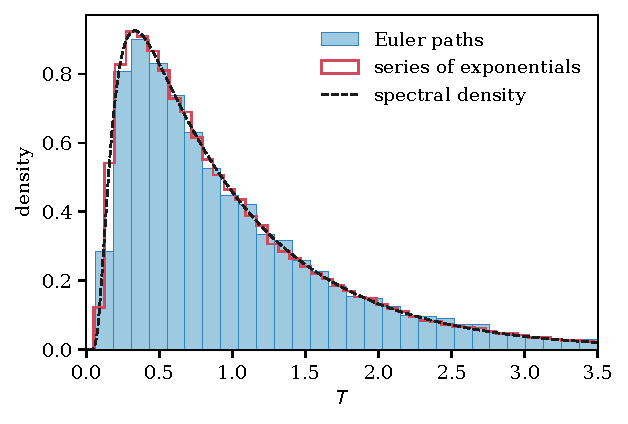
\includegraphics[width=0.92\textwidth]{exit_time}
\caption{The exit time of Brownian motion from $(-1,1)$. Histograms of 6000 paths simulated by the Euler scheme with step $2\times10^{-4}$ and of 60000 draws of the series of exponentials of Theorem~\ref{thm:exit_series} truncated at 200 terms, and the density of the theorem summed over 200 terms.}
\label{fig:exit}
\end{figure}

The theorem is a special case of a general principle due to Kent~\cite{kent1980}. For a regular one dimensional diffusion started at a reflecting or entrance boundary $a$, the hitting time of a level $b$ is distributed as $\sum_n E_n/\lambda_n$, where $0<\lambda_1<\lambda_2<\cdots$ are the eigenvalues of minus the generator on $(a,b)$ with Dirichlet condition at $b$ and the natural condition at $a$. Hitting times are therefore infinitely divisible, indeed generalized Gamma convolutions in the sense of Chapter~\ref{ch:mixtures}, and their L\'evy measures are determined by the spectrum. Krein's theory of strings, in the form given by Kotani and Watanabe~\cite{kotani1982}, runs the other way: a diffusion in natural scale with given boundary conditions is determined by its spectral measure, which records the eigenvalues together with their norming constants. The companion volume~\cite{polsonh8} uses this inverse spectral correspondence for the Riemann $\xi$ function of Section~\ref{sec:excursions_xi}.

\section{Brownian excursions and the Riemann \texorpdfstring{$\xi$}{xi} function}
\label{sec:excursions_xi}

One identity of the Yor school connects Brownian motion with the Riemann zeta function. Let $\xi(s) = \frac12 s(s-1)\pi^{-s/2}\Gamma(s/2)\zeta(s)$ be the Riemann $\xi$ function, entire and symmetric under $s\mapsto1-s$, and let $\Xi(x) = \xi(\frac12+ix)$ be its restriction to the critical line, an even entire function that is real for real $x$.

\begin{theorem}[Biane, Pitman and Yor]
\label{thm:bpy}
Let $m$ be the maximum of a standard Brownian excursion of unit length and $Y = \sqrt{2/\pi}\,m$. Then for all $s\in\C$,
\[
\E\big[Y^s\big] = 2\,\xi(s).
\]
\end{theorem}

We quote the theorem without proof; the proof in~\cite{bpy2001} expresses the law of $m$ through the Jacobi theta function, whose functional equation is the source of the functional equation of $\xi$. The identity says that the Riemann hypothesis, the statement that the zeros of $\xi$ lie on $\Re s = \frac12$, is a statement about the Mellin transform of a Brownian functional. It is the bridge between the two Hilbert problems of this book and its companion, and we return to it in Chapter~\ref{ch:open}.

\section{Matrix Brownian motion and Wick rotation}

Let $X_t$ be Brownian motion on the space of $n\times n$ Hermitian matrices, with independent Brownian diagonal entries of variance $t$ and independent real and imaginary parts of the off diagonal entries, each of variance $t/2$. Dyson showed in 1962~\cite{dyson1962} that its eigenvalues $x_1<\cdots<x_n$ evolve as
\[
\dd x_i = \dd W_i + \sum_{j\neq i}\frac{\dd t}{x_i-x_j},
\]
where $W_1,\dots,W_n$ are independent standard Brownian motions, a system of Brownian particles with logarithmic repulsion that never collide. Biane~\cite{biane2009} gives a geometric description, by a Doob transform, of the motion of the eigenvalues or singular values of Brownian motions on Hermitian, complex invertible and unitary matrices. In a second, largely independent part Biane looks again at a paper of P\'olya of 1926~\cite{polya1926}, which introduces a function close to the Riemann $\xi$ function and shows that it satisfies the Riemann hypothesis, and observes that both functions have an interpretation through Mellin transforms of first passage times of diffusions. Replacing the time $t$ by the imaginary time $it$, the Wick rotation, turns the heat semigroup $e^{t\Delta/2}$ into the Schr\"odinger group $e^{it\Delta/2}$. Chapter~\ref{ch:quantum} uses this rotation to pass between Brownian motion and quantum mechanics.

\section{Bachelier's maximum and the reflection principle}

Bachelier computed in 1900~\cite{bachelier1900} the law of the maximum of his price process.

\begin{theorem}[Reflection principle]
\label{thm:reflection}
Let $B$ be standard Brownian motion, $M_t = \sup_{s\leq t}B_s$ and $a>0$. Then $\P(M_t\geq a) = 2\P(B_t\geq a)$, so $M_t\eqd|B_t|$. More precisely, for $b\leq a$,
\[
\P(M_t\geq a,\,B_t\leq b) = \P(B_t\geq2a-b).
\]
\end{theorem}

\begin{proof}
Let $\tau_a = \inf\{s:B_s = a\}$, a stopping time. By the strong Markov property, $(B_{\tau_a+s}-a)_{s\geq0}$ is a Brownian motion independent of $\mathcal{F}_{\tau_a}$, and so is its negative. Reflecting the path after $\tau_a$ maps $\{M_t\geq a,B_t\leq b\}$ bijectively, and measure preservingly, onto $\{B_t\geq2a-b\}$. Taking $b = a$ and adding $\P(B_t\geq a)$ gives the first identity.
\end{proof}

Differentiating gives the joint density of $(M_t,B_t)$, and with it the density of the hitting time $\tau_a$:
\[
\P(\tau_a\in\dd t) = \frac{a}{\sqrt{2\pi t^3}}e^{-a^2/2t}\dd t,
\]
the L\'evy law, a positive stable law of index one half. It is an HCM law and therefore a GGC, with Laplace transform $e^{-a\sqrt{2\lambda}}$. Bachelier used the reflection argument, informally, to price barrier type contracts.

\section{L\'evy's arcsine laws}

Let $O_t = \int_0^t\mathbb{1}\{B_s>0\}\dd s$ be the time Brownian motion spends positive up to time $t$, and $g_t = \sup\{s\leq t:B_s = 0\}$ the last zero before $t$. L\'evy proved that $O_1$ and $g_1$ both have the arcsine law with density $\frac{1}{\pi\sqrt{x(1-x)}}$ on $(0,1)$. The law is symmetric and concentrated near the endpoints: a Brownian path typically spends most of its time on one side. The arcsine law is a Beta$(\frac12,\frac12)$ law, which reappears in Chapter~\ref{ch:mixtures} as the law of the shrinkage coefficient of the horseshoe prior. If $N_1$ and $N_2$ are independent standard normal variables, then $N_1^2$ and $N_2^2$ are independent Gamma variables with shape $\frac12$ and the same scale, so $N_2^2/(N_1^2+N_2^2)$ has the Beta$(\frac12,\frac12)$ law. The half Cauchy local scale of the horseshoe is $\lambda = |N_1|/|N_2|$, and its shrinkage coefficient $1/(1+\lambda^2)$ is exactly this ratio.

\section{It\^o's formula and Girsanov's theorem}

For a semimartingale $X$ and a twice continuously differentiable $f$, It\^o's formula reads
\[
f(X_t) = f(X_0)+\int_0^tf'(X_s)\dd X_s+\frac12\int_0^tf''(X_s)\dd\langle X\rangle_s.
\]
Girsanov's theorem describes how the law of Brownian motion changes under a change of drift.

\begin{theorem}[Girsanov]
Let $b$ be a bounded progressively measurable process and define $G_t = \exp\big(\int_0^tb_s\dd B_s-\frac12\int_0^t|b_s|^2\dd s\big)$. Under the measure $\dd\mathbb{Q} = G_T\dd\P$ on $\mathcal{F}_T$, the process $\tilde B_t = B_t-\int_0^tb_s\dd s$ is a Brownian motion on $[0,T]$.
\end{theorem}

We quote the theorem without proof; see Chapter VIII of~\cite{revuzyor}, or Girsanov's original paper~\cite{girsanov1960}. Since $b$ is bounded, Novikov's criterion applies, so $G$ is a martingale with $\E G_T = 1$ and $\mathbb{Q}$ is a probability measure. Girsanov's density is a likelihood ratio between path measures, and its logarithm is the log likelihood of the drift. For a diffusion $\dd X = b_\theta(X)\dd t+\dd B$ observed continuously, the likelihood of $\theta$ relative to the driftless process is
\[
L(\theta) = \exp\Big(\int_0^Tb_\theta(X_s)\dd X_s-\frac12\int_0^T|b_\theta(X_s)|^2\dd s\Big),
\]
and Bayesian inference for diffusions, as in Polson and Roberts~\cite{polsonroberts1994}, starts from this formula. Let $b$ and $b'$ be bounded progressively measurable drifts, and let $\P^b$ and $\P^{b'}$ be the laws of the solutions of $\dd X = b_s\dd t+\dd B$ and $\dd X = b'_s\dd t+\dd B$ with the same initial condition and unit diffusion coefficient. The relative entropy of $\P^b$ with respect to $\P^{b'}$ is $\frac12\E^b\int_0^T|b_s-b'_s|^2\dd s$, where $\E^b$ is the expectation under $\P^b$. This is the identity behind the Schr\"odinger bridge computations of Chapter~\ref{ch:gbc} and the Donsker Varadhan rate function of Chapter~\ref{ch:quantum}.

\section{Local time and the Ray Knight theorems}

Brownian motion in one dimension has a local time $L_t^x$, jointly continuous in $(t,x)$, such that $\int_0^tf(B_s)\dd s = \int f(x)L^x_t\dd x$ for all bounded measurable $f$. The Ray Knight theorems identify the local time as a function of the space variable, at suitable random times, with squared Bessel processes; see Chapter XI of~\cite{revuzyor}. For instance, if $\tau_a$ is the hitting time of $a>0$, then $(L^{a-x}_{\tau_a})_{0\leq x\leq a}$ is a squared Bessel process of dimension two started at zero, so that $L^{a-x}_{\tau_a}$ is exponential with mean $2x$, and $(L^{-y}_{\tau_a})_{y\geq0}$ is a squared Bessel process of dimension zero started at $L^0_{\tau_a}$. The additivity of squared Bessel processes then explains why local times at hitting times are infinitely divisible. They are Gamma convolutions only on the first range. For $y>0$ the law of $L^{-y}_{\tau_a}$ has Laplace transform $(1+2\lambda y)/(1+2\lambda(y+a))$ and an atom of mass $y/(a+y)$ at zero, which a Gamma convolution does not have. Biane, Pitman and Yor~\cite{bpy2001} use the Ray Knight theorems and symmetries of Brownian paths to give direct arguments for many of the coincidences in law between Brownian functionals that they tabulate. For some of the coincidences no direct argument is known, and some of these are equivalent to the functional equation of the Jacobi theta function.

\section*{Exercises}
\begin{enumerate}
\item Show that the L\'evy Ciesielski series truncated after level $n$ agrees with the full series at the dyadic points $k2^{-(n+1)}$ and is linear in between.
\item Use the reflection principle to derive the density of $\tau_a$ and verify that its Laplace transform is $e^{-a\sqrt{2\lambda}}$.
\item From \eqref{eq:exit_laplace}, compute $\E T$ and $\Var T$ for the exit time from $(-1,1)$, and check them against the series of exponentials.
\item Show that the exit time from $(-a,a)$ of Brownian motion started at zero has the law of $a^2T$, and deduce its Laplace transform.
\item Simulate the Dufresne perpetuity by Euler discretization for $\mu = 1$ and compare with the law of $1/(2\gamma_1)$. Compare quantiles, since this law has an infinite mean.
\end{enumerate}


\section*{Notes}

Nelson's \emph{Dynamical Theories of Brownian Motion}~\cite{nelson1967} remains the best short account of Einstein, Langevin and Ornstein Uhlenbeck. Revuz and Yor~\cite{revuzyor} is the standard reference for Bessel processes and time change.
